\chapter{Opis rada sistema}\label{sistem}
U ovom poglavlju se detaljno izlaže opis rada sistema iz dve perspektive: perspektive studenta - korisnika sistema, i perspektive profesora - administratora sistema.

\section{Opis rada sistema iz perspektive studenta}
\subsection{Logovanje na sistem i registracija}
Prva stranica koja se prikazuje kada korisnik uputi pretraživač na adresu servisa jeste login stranica (URI: \texttt{/login}), prikazana na slici \ref{fig:login}. Na ovoj stranici korisnik unosi svoju email adresu i lozinku i nakon toga se loguje na sistem pritiskom na dugme \textbf{Prijava}. Prihvataju se samo email adrese koje se završavaju sa \texttt{@etf.rs}. Email adresa se dinamički proverava dok je korisnik unosi, i to tako da je dugme za prijavu onemogućeno dok se ne unese korektna adresa. Pokušaj prijave korisnika koji nije registrovan, ili koji se ulogovao sa pogrešnom lozinkom se prikazuju kao greška (slika \ref{fig:login-error}).

Novi korisnici mogu da se registruju pritiskom na dugme \textbf{Registracija}. Ta akcija ih vodi na stranicu za registrovanje novih korisnika (URI: \texttt{/register}, slika \ref{fig:register}), koja od korisnika traži da unese email adresu. Ista ograničenja vezana za email adresu se primenjuju i ovde. Pokušaj postojećeg korisnika da se ponovo registruje rezultuje greškom. Nakon što unese email, pritiskom na dugme \textbf{Izvrši} se korisnik registruje na sistem. Nakon uspešne registracije korisniku se prikazuje stranica sa slike \ref{fig:register-success}. Tom prilikom se na unetu email adresu automatski šalje email sa nasumično generisanom lozinkom za tog korisnika. Sa ovom lozinkom korisnik sada može da se uloguje na sistem preko stranice za logovanje.
\begin{figure}[p]
\centering
\fbox{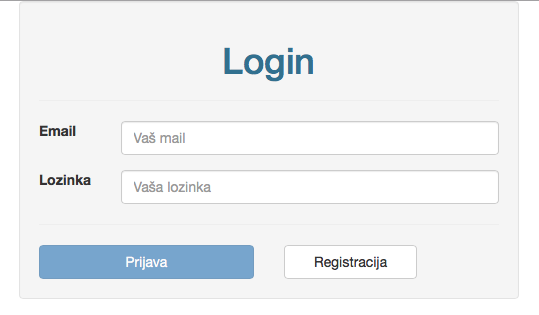
\includegraphics[width=0.45\textwidth]{login}
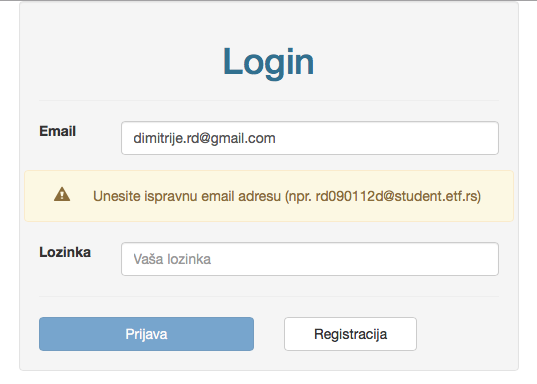
\includegraphics[width=0.45\textwidth]{login-wrongemail}}
\caption{\textit{Levo}: inicijalni izgled login stranice, \textit{desno}: login stranica tokom unosa email adrese}
\label{fig:login}
\end{figure}
\begin{figure}[p]
\centering
\fbox{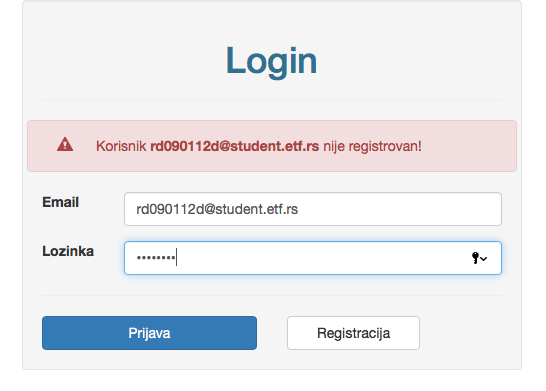
\includegraphics[width=0.45\textwidth]{login-error-unknown}
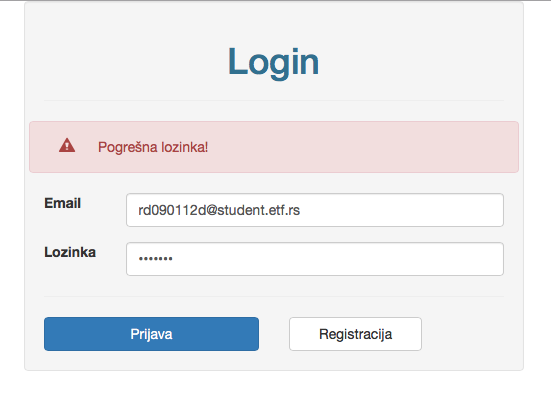
\includegraphics[width=0.45\textwidth]{login-error-password}}
\caption{\textit{Levo}: izgled login stranice nakon što neregistrovani korisnik pokuša da se uloguje, \textit{desno}: izgled login stranice ukoliko korisnik unese pogrešnu lozinku}
\label{fig:login-error}
\end{figure}
\begin{figure}[p]
\centering
\fbox{
\includegraphics[width=0.45\textwidth]{register}
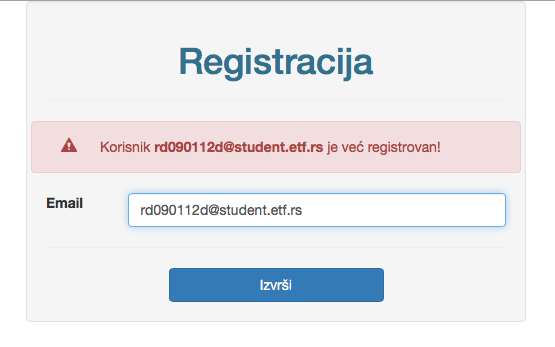
\includegraphics[width=0.45\textwidth]{register-error}}
\caption{\textit{Levo}: inicijalni izgled stranice za registrovanje, \textit{desno}: stranica za registracije nakon što već registrovani korisnik pokuša da se registruje}
\label{fig:register}
\end{figure}
\begin{figure}[ht]
\centering
\fbox{
\includegraphics[width=0.95\textwidth]{register-success}}
\caption{Izgled stranice za registraciju nakon uspešne registracije}
\label{fig:register-success}
\end{figure}

\subsection{Stranica sa pregledom testova}
Nakon uspešne prijave na sistem, korisniku se prikazuje stranica sa pregledom svih testova trenutno u sistemu (URI: \texttt{/user}, slike \ref{fig:assignments} i \ref{fig:assignments-collapsed}). Ova stranica se prikazuje i kao početna stranica ukoliko je korisnik već ulogovan na sistem, a pregledač usmeri na \textit{root} URL servisa. Testovi su grupisani po kategorijama, i prikazani unutar tabele u svakoj kategoriji. Zaglavlja tabele sadrže imena kategorija i predstavljaju interaktivne linkove, koji na klik proširuju svoj sadržaj, tj. telo tabele sa testovima.

Za svaki test se prikazuje ime testa, broj stranica sa pitanjima, i ukupan broj pitanja. Testovi koji se prikazuju na ovoj stranici se dele na:
\begin{itemize}
\renewcommand\labelitemi{--}
\item \textbf{Završene testove}, tj. testove koje je korisnik predao. Za ove testove se dodatno prikazuju datum i vreme kada je test započet, datum i vreme kada je test završen, i ocena, u vidu procenta tačnih odgovora u odnosu na ukupan broj pitanja. Boja pozadine ovih unosa je zelena.
\item \textbf{Testove u toku}, tj. testove koje je korisnik započeo, ali nije završio. Za ove testove se dodatno prikazuju datum i vreme kada je test započet, procenat od ukupnog broja pitanja na koja je student dao odgovor, tj. progres, i link ka stranici sa testom. Boja pozadine ovih unosa je žuta.
\item \textbf{Nezapočete testove}, tj. testove koje korisnik nikada nije polagao. Za ove testove se dodatno prikazuje link ka stranici sa testom i prazan progres. Boja pozadine ovih unosa je bela.
\end{itemize}
\begin{figure}[p]
\centering
\fbox{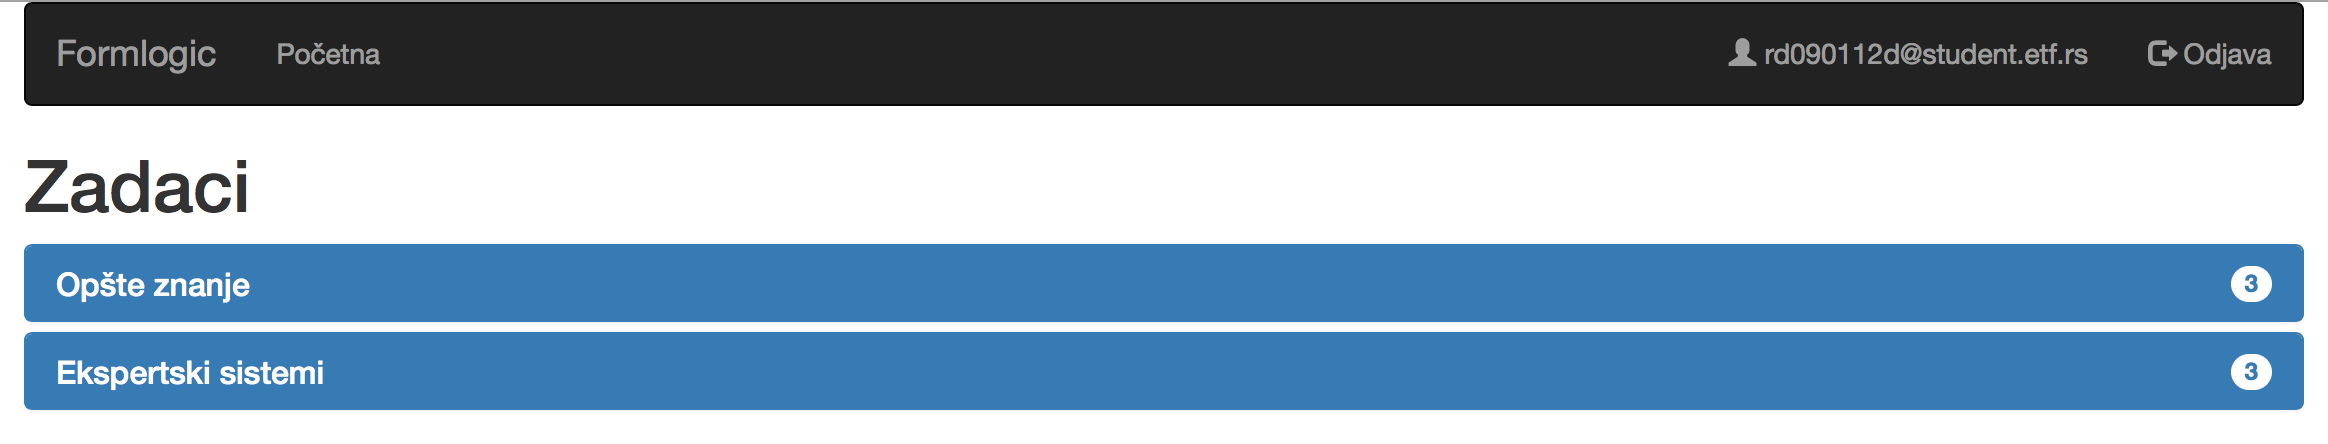
\includegraphics[width=0.95\textwidth]{assignments}}
\caption{Inicijalni izgled stranice sa zadacima, sa izlistanim kategorijama (broj testova unutar kategorije je naznačen sa desne strane interaktivnog linka)}
\label{fig:assignments}
\end{figure}
\begin{figure}[p]
\centering
\fbox{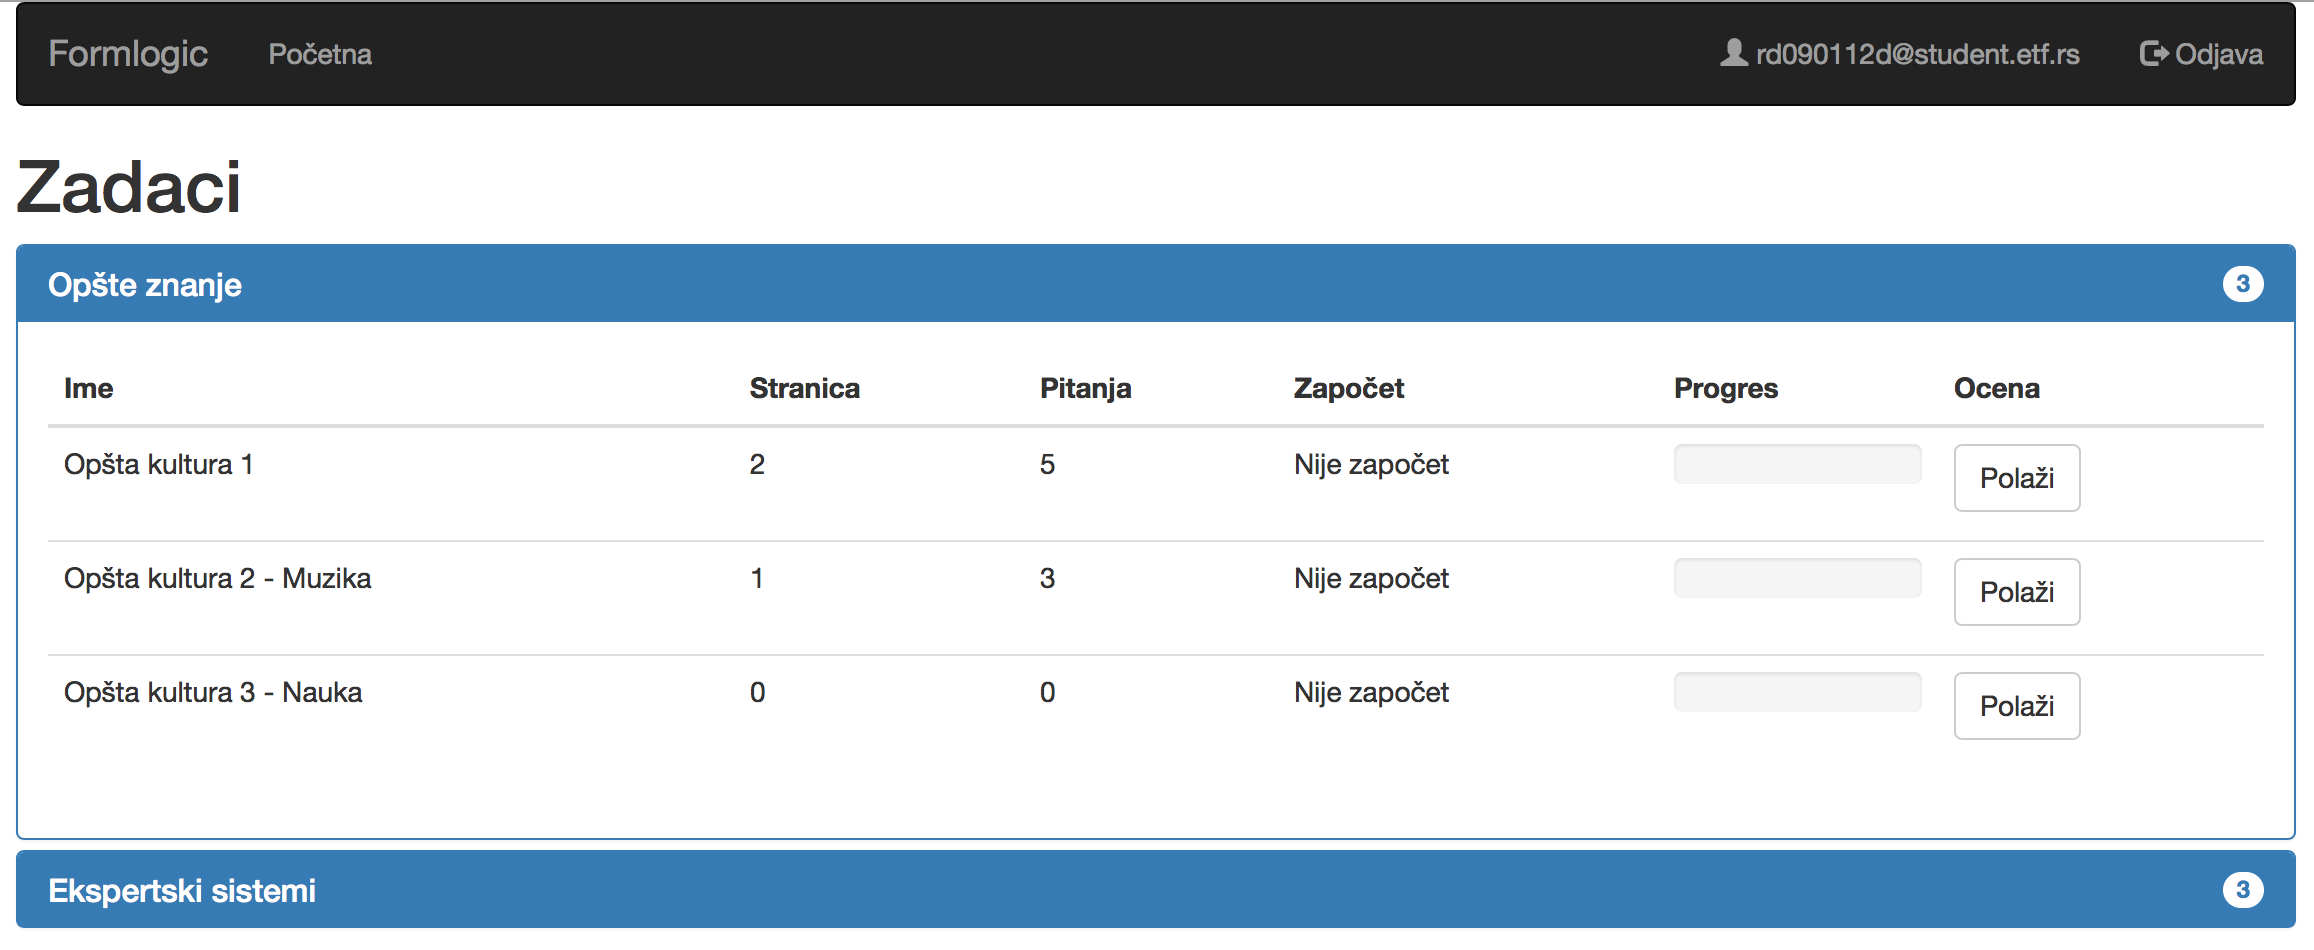
\includegraphics[width=0.95\textwidth]{assignments-collapsed}}
\fbox{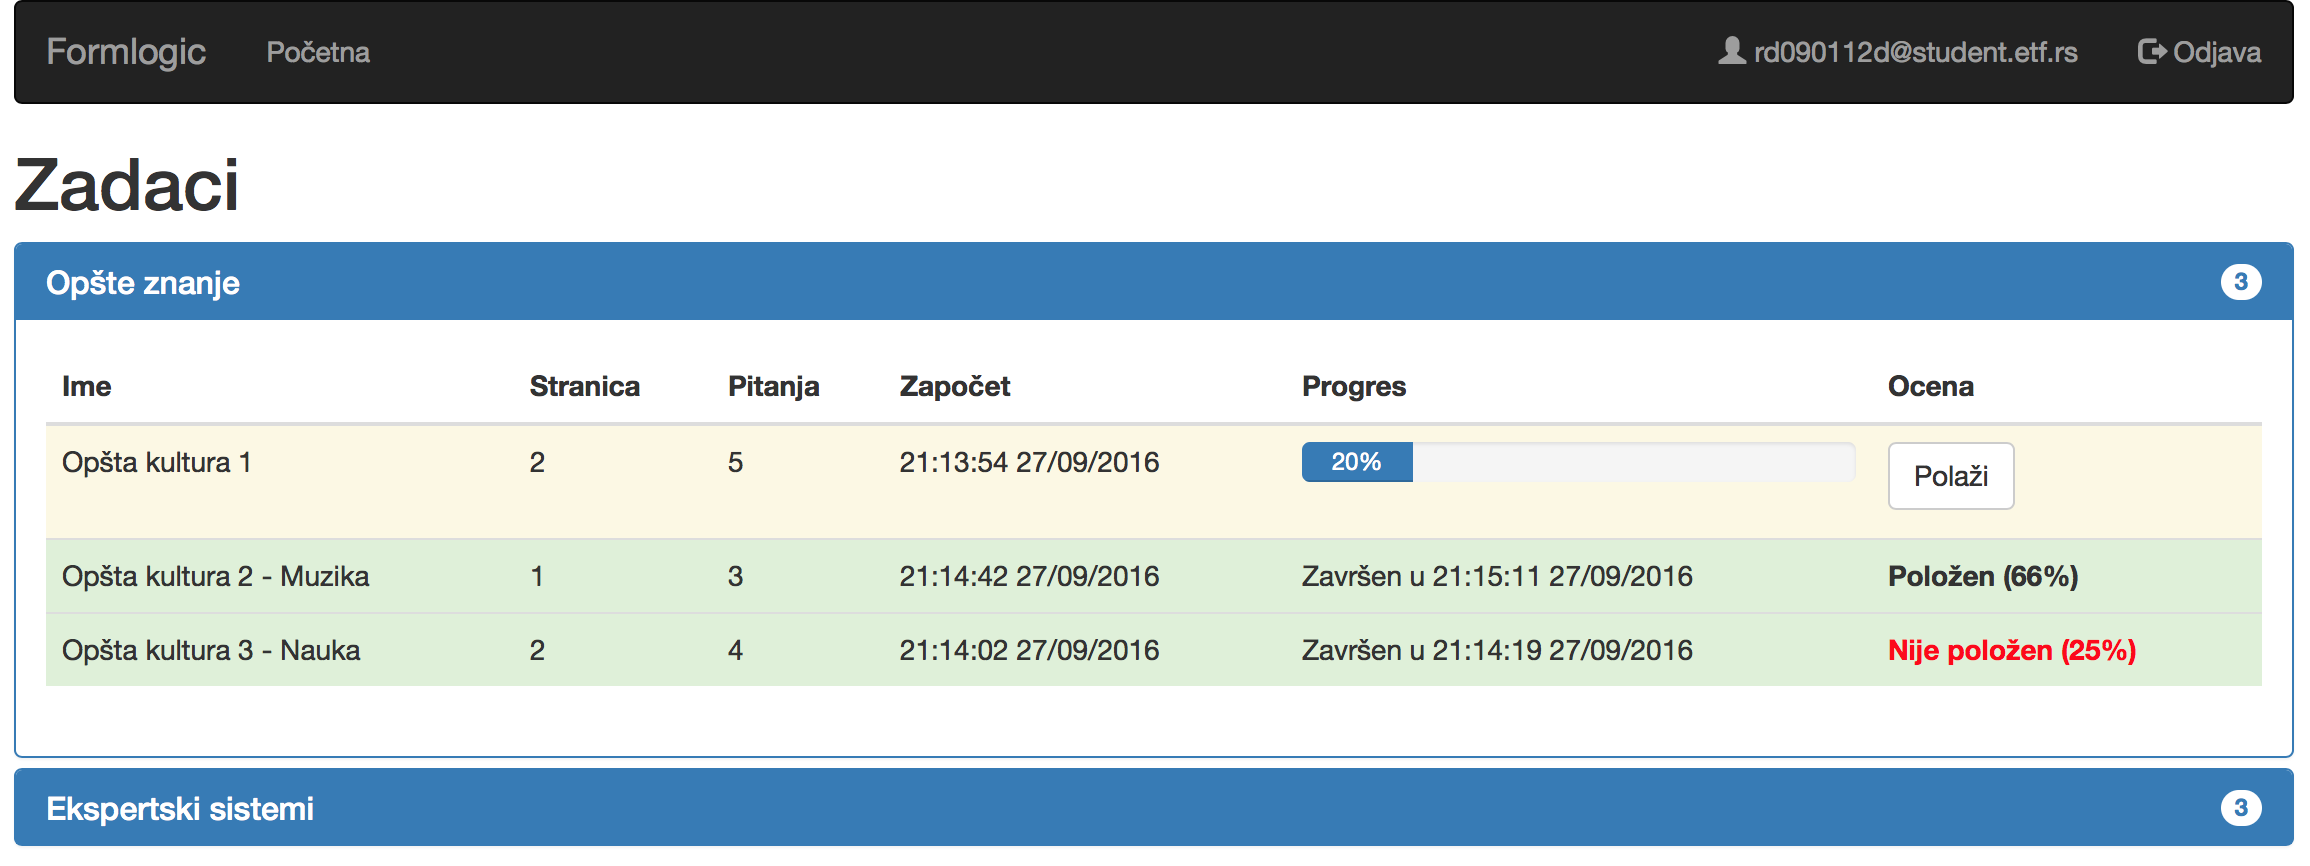
\includegraphics[width=0.95\textwidth]{assignments-collapsed-progress}}
\caption{\textit{Gore}: stranica sa zadacima nakon što je sadržaj prve kategorije proširen, za korisnika koji nije polagao nijedan test, \textit{dole}: stranica sa zadacima sa prvim testom u toku, položenim drugim testom i nepoloženim trećim testom}
\label{fig:assignments-collapsed}
\end{figure}

Nakon što korisnik klikne na dugme \textbf{Polaži}, prikazuje mu se prva stranica sa pitanjima odabranog testa. Kada korisnik prvi put otvori stranicu sa pitanjima nekog testa, smatra se da je otpočeo proces izrade tog testa, te će unos u tabeli testova za taj test od tada biti označen žutom pozadinom.

\subsection{Stranica sa pitanjima}
\label{section:submit}
URI stranice sa pitanjima je sledećeg oblika:
\begin{verbatim}
/user/progress/<assignment-id>/<page-ord>
\end{verbatim}
gde je \texttt{assignment-id} ID zadatka, a \texttt{page-ord} redni broj stranice sa pitanjima tog zadatka. Redni brojevi stranica počinju od broja 1.

Stranica sa pitanjima sastoji se od tri dela (slika \ref{fig:task}). Prvi deo je zaglavlje stranice, na kome se nalazi ime testa, redni broj trenutne stranice sa pitanjima, ukupan broj stranica sa pitanjima u testu i progres popunjavanja testa, u procentima. Progres se računa na osnovu broja popunjenih pitanja, tako da korisnik može da primeti ukoliko je slučajno preskočio neko pitanje sa prethodnih stranica pre nego što preda test.
\begin{figure}[h]
\centering
\fbox{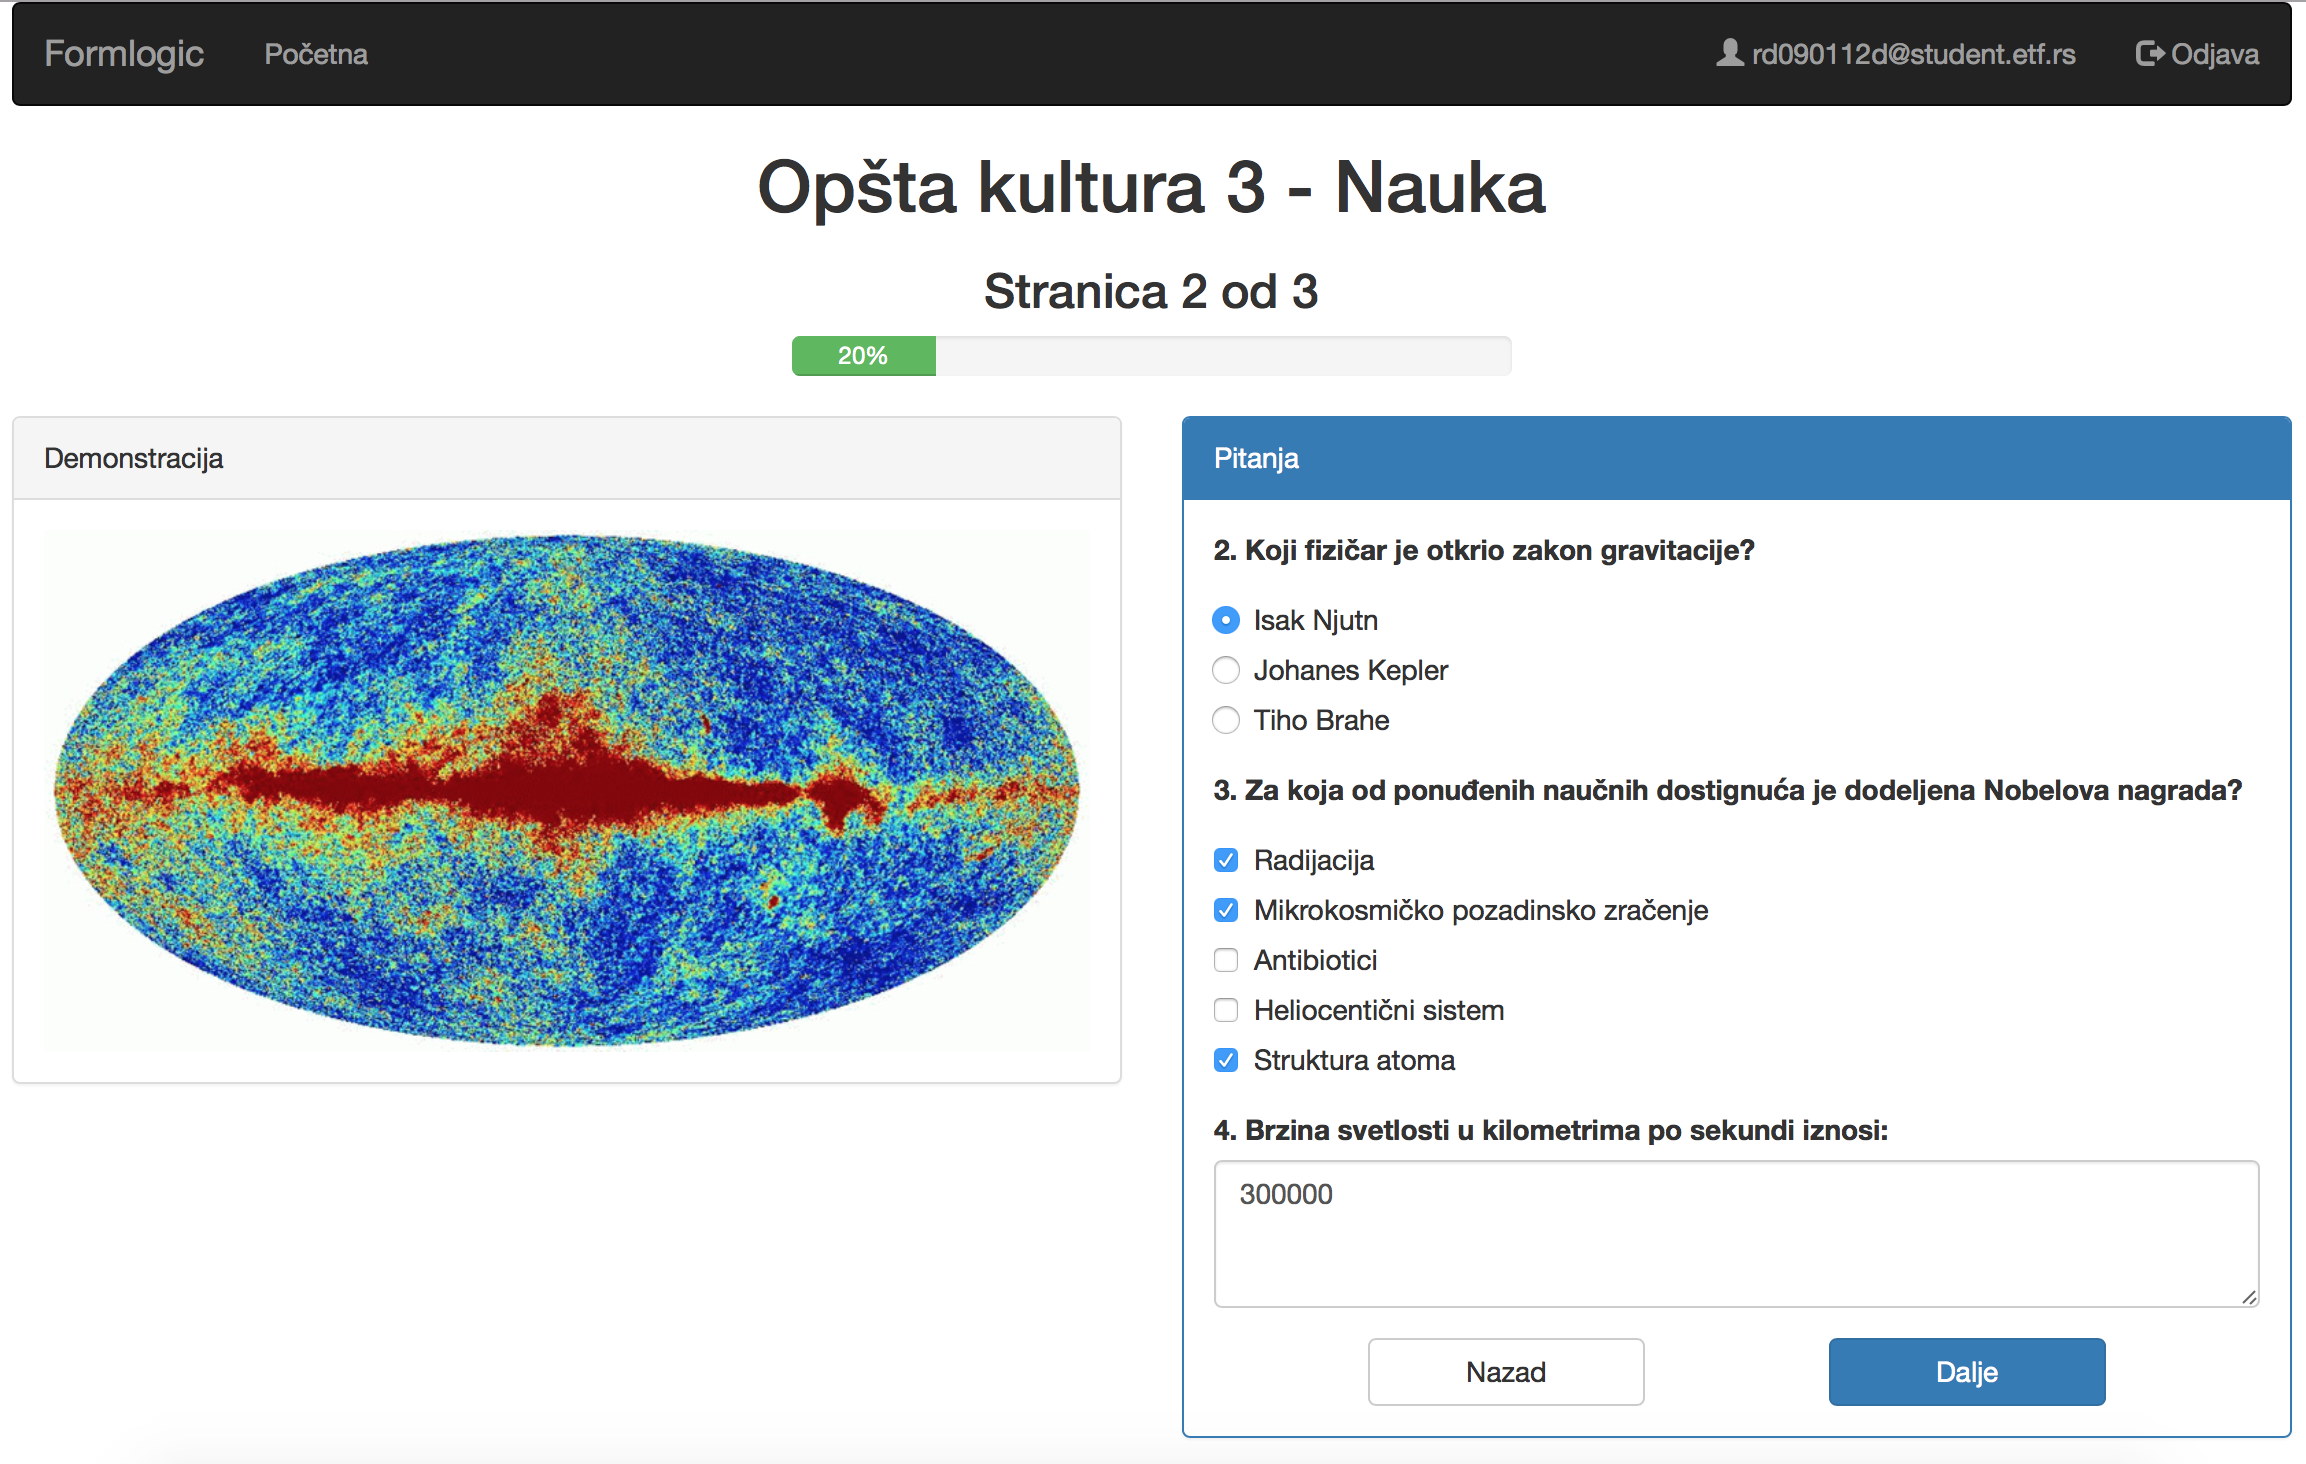
\includegraphics[width=0.95\textwidth]{task}}
\caption{Izgled stranice sa pitanjima sa popunjenim odgovorima}
\label{fig:task}
\end{figure}

Drugi deo stranice sa pitanjima je deo sa demonstracijom. Ovaj opcioni deo se nalazi u panelu sa leve strane i sadrži proizvoljan sadržaj. Sadržaj se može specificirati za svaku stranicu sa pitanjima ponaosob, i unosi se direktno u bazu, zajedno sa ostalim informacijama vezanim za konkretni test. Sadržaj se navodi kao deo izvornog koda u Clojure-u, koji se interpretira i renderuje zajedno sa ostatkom HTML stranice, tako da je ovim putem moguće vršiti i složenije operacije nad sadržajem koji treba prikazati.

Treći deo stranice sa pitanjima su sama pitanja. Ona se nalaze u panelu sa desne strane. Na jednoj stranici sa pitanjima moguće je imati proizvoljan broj pitanja. Pitanja su navedena jedna ispod drugog, u rastućem redosledu rednog broja pitanja. Kada se stranica učita, odgovor na svako pitanje je nepopunjen. Kada korisnik jednom odgovori na pitanja sa jednim ili više ponuđenih odgovora, više nije u mogućnosti da poništi svoj odgovor i vrati pitanje u nepopunjeno stanje. Nakon svih pitanja, na dnu panela se nalaze dva dugmeta: \textbf{Nazad} i \textbf{Dalje}. Prvo dugme služi da se korisnik vrati na prethodnu stranicu sa pitanjima, a potonje dugme služi da se ode na sledeću stranicu sa pitanjima. U oba slučaja se čuvaju odgovori koje je korisnik dao na trenutnoj stranici.

Kada se korisnik nađe na poslednjoj stranici sa pitanjima, na dnu stranice pojavljuje se dugme \textbf{Predaj}. Nakon pritiska na ovo dugme korisniku se prikazuje modalni dijalog koji upozorava na to da akcija predavanja testa ne može da se poništi, dajući korisniku još jednu šansu da proveri svoje odgovore (slika \ref{fig:task-submit}. Ukoliko korisnik u pomenutom dijalogu potvrdi akciju predaje, test se smatra završenim, a korisnik se vraća na stranicu sa pregledom testova. Od ovog trenutka korisnik više nije u mogućnosti da menja odgovore na pitanja ovog testa, niti da ga ponovo polaže.

Ukoliko korisnik prekine polaganje u bilo kom trenutku, na primer tako što zatvori prozor pregledača ili ode na neku drugu internet stranicu, može nastaviti sa polaganjem tako što će izabrati test čije je polaganje prekinuo sa stranice sa pregledom testova. Dotadašnji progres, tj. odgovori koje je korisnik dao pre nego što je prekinuo polaganje, će biti restaurirani.
\begin{figure}[h]
\centering
\fbox{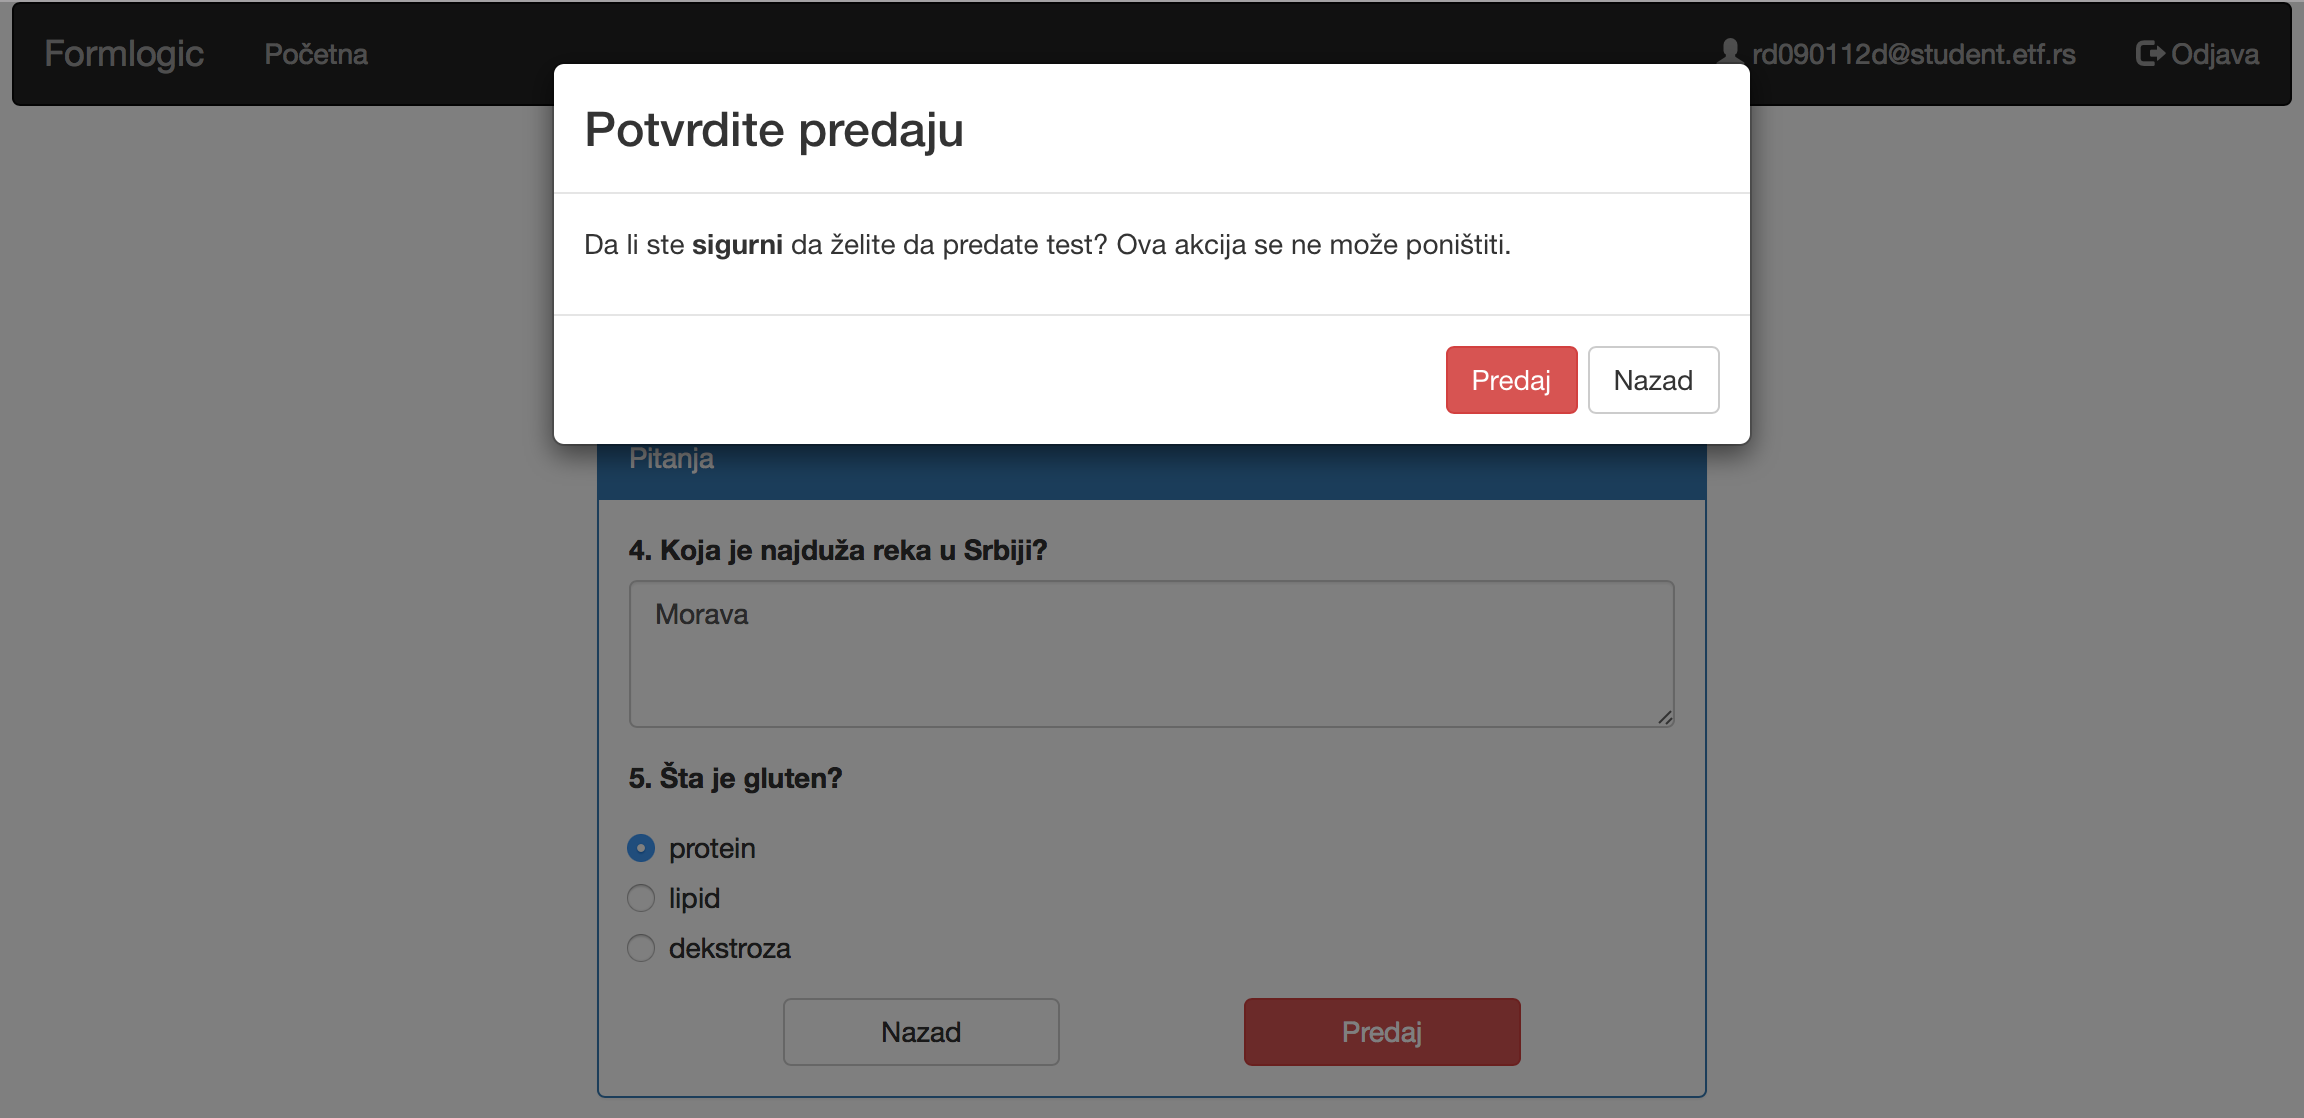
\includegraphics[width=0.95\textwidth]{task-submit}}
\caption{Izgled dijaloga za potvrdu predaje testa}
\label{fig:task-submit}
\end{figure}

\subsection{Primer demonstracije: svođenje na KNF}
Kao jedan primer onoga šta panel sa demonstracijom može da sadrži izrađena je demonstracija svođenja logičkog izraza u KNF formu (slika \ref{fig:cnf}). Panel sadrži tekstualno polje u kome korisnik unosi formulu (za korišćenu sintaksu pogledati sekciju \ref{sec:syntax}). Nakon unosa formula, pritiskom na dugme \textbf{Pošalji}, uneta formula se preko AJAX POST zahteva šalje serveru, koji je svodi na KNF i rezultat vraća u JSON obliku. Rezultat se, po koracima, renderuje kao \LaTeX \space jednačina.
\begin{figure}[h]
\centering
\fbox{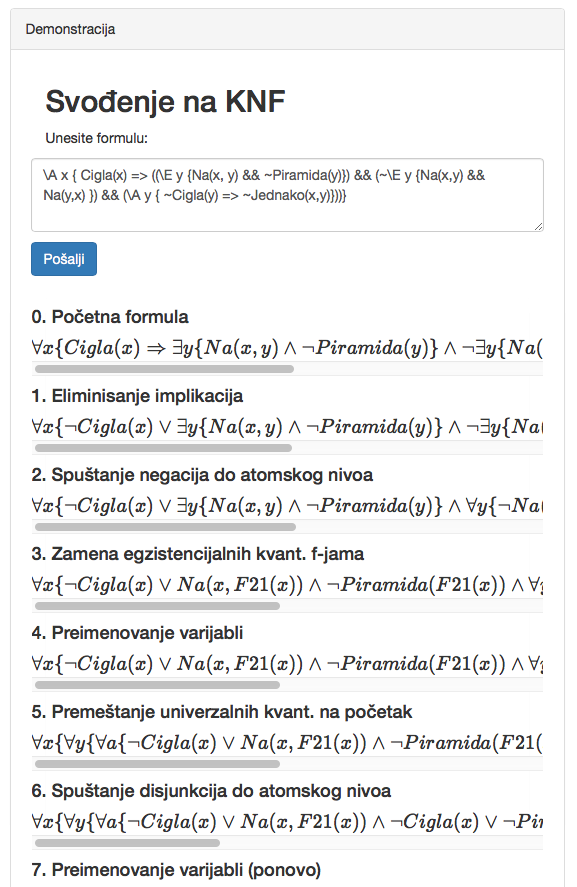
\includegraphics[width=0.45\textwidth]{cnf}
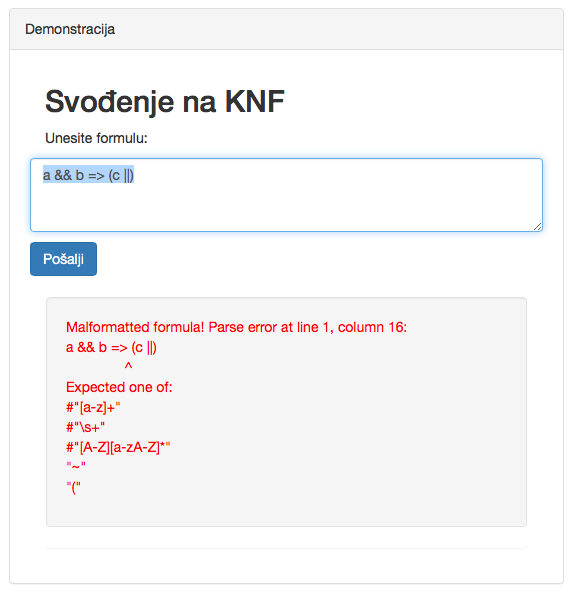
\includegraphics[width=0.45\textwidth]{cnf-error}}
\caption{\textit{Levo}: izgled panela sa demonstracijom algoritma svođenja na KNF, \textit{desno}: izgled istog panela u slučaju greške u sintaksi formule}
\label{fig:cnf}
\end{figure}
Ukoliko sintaksa formule nije ispravna, korisniku se prikazuje greška, zajedno sa informacijom o problematičnom delu formule.

Sadržaj celog panela se realizuje kao poziv Clojure funkcije \texttt{views/cnf-page}, unutar kolone sa sadržajem u odgovarajućoj tabeli (pogledati sekciju \ref{sec:panel-contents}).

\section{Opis rada sistema iz perspektive profesora}
\subsection{Stranica za pretraživanje završenih testova}
Nakon uspešnog logovanja na sistem, administratorima se prikazuje stranica za pretraživanje i pregled odrađenih testova (URI: \texttt{/user}, slika \ref{fig:assignments-admin}). Ova stranica je podeljena na dva dela. Prvi deo se koristi za pretragu testova preko email naloga studenata, a drugi deo se koristi za pretragu testova po oblastima. Prelaz između ove dve stranice vrši se odabirom zaliska pri vrhu strane.

\begin{figure}[h]
\centering
\fbox{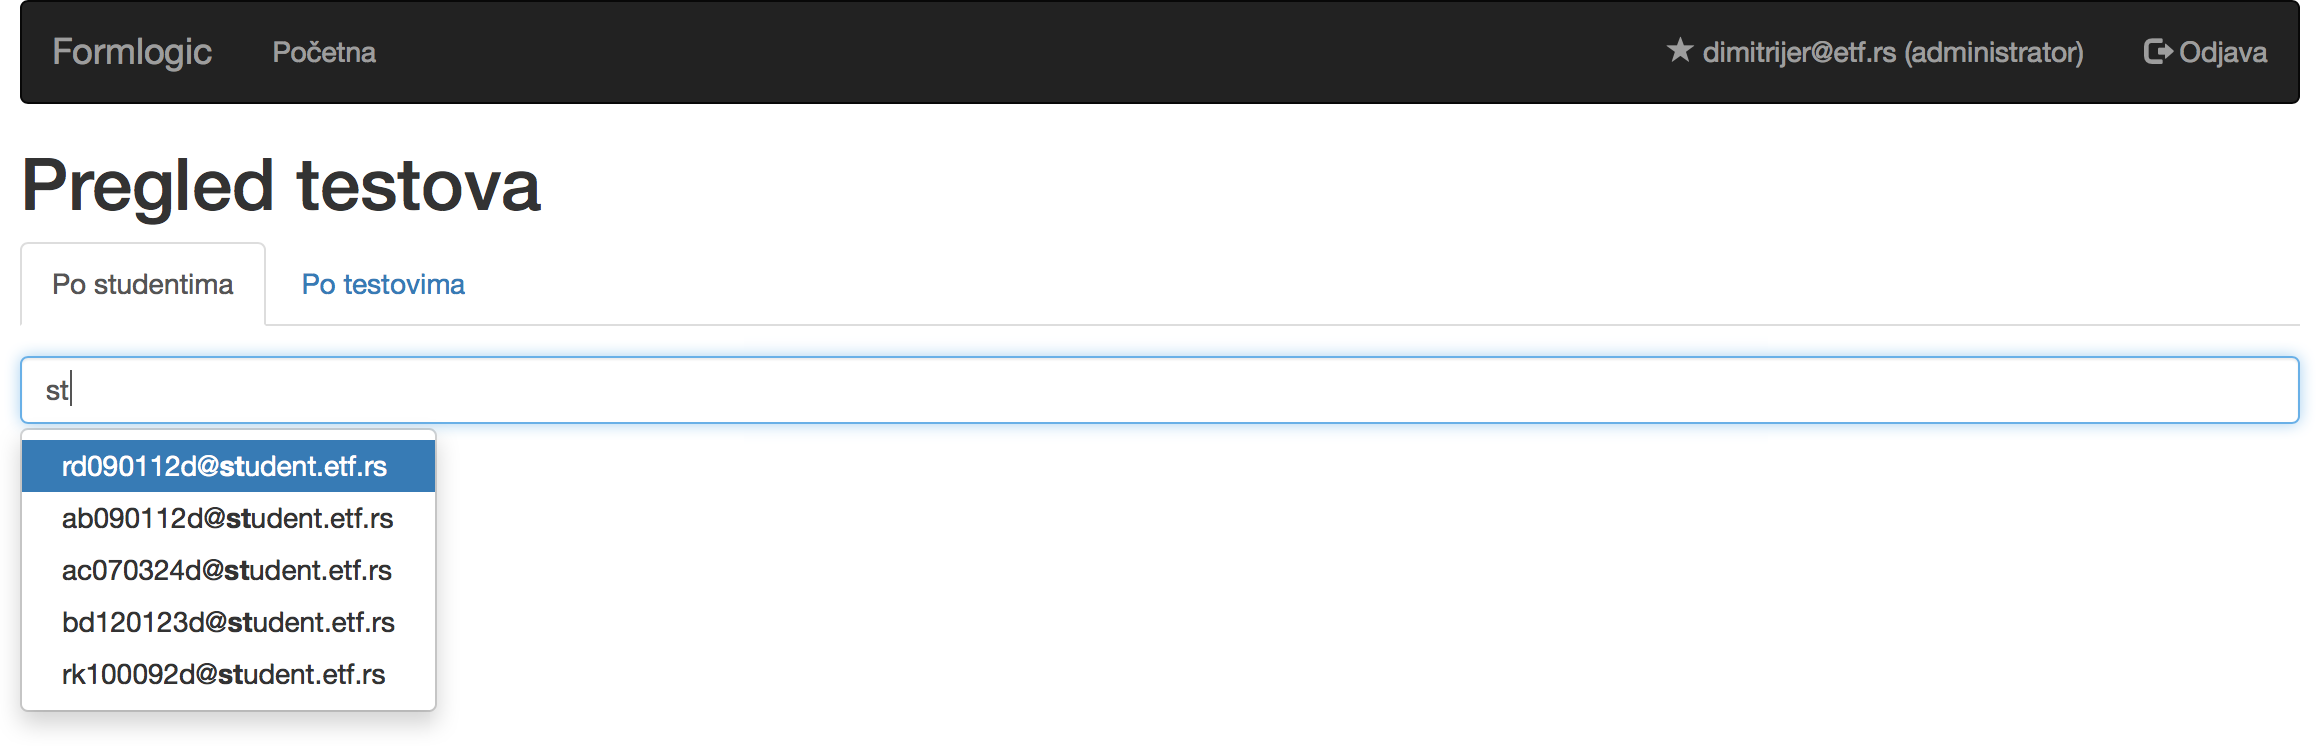
\includegraphics[width=0.95\textwidth]{assignments-admin-students}}
\fbox{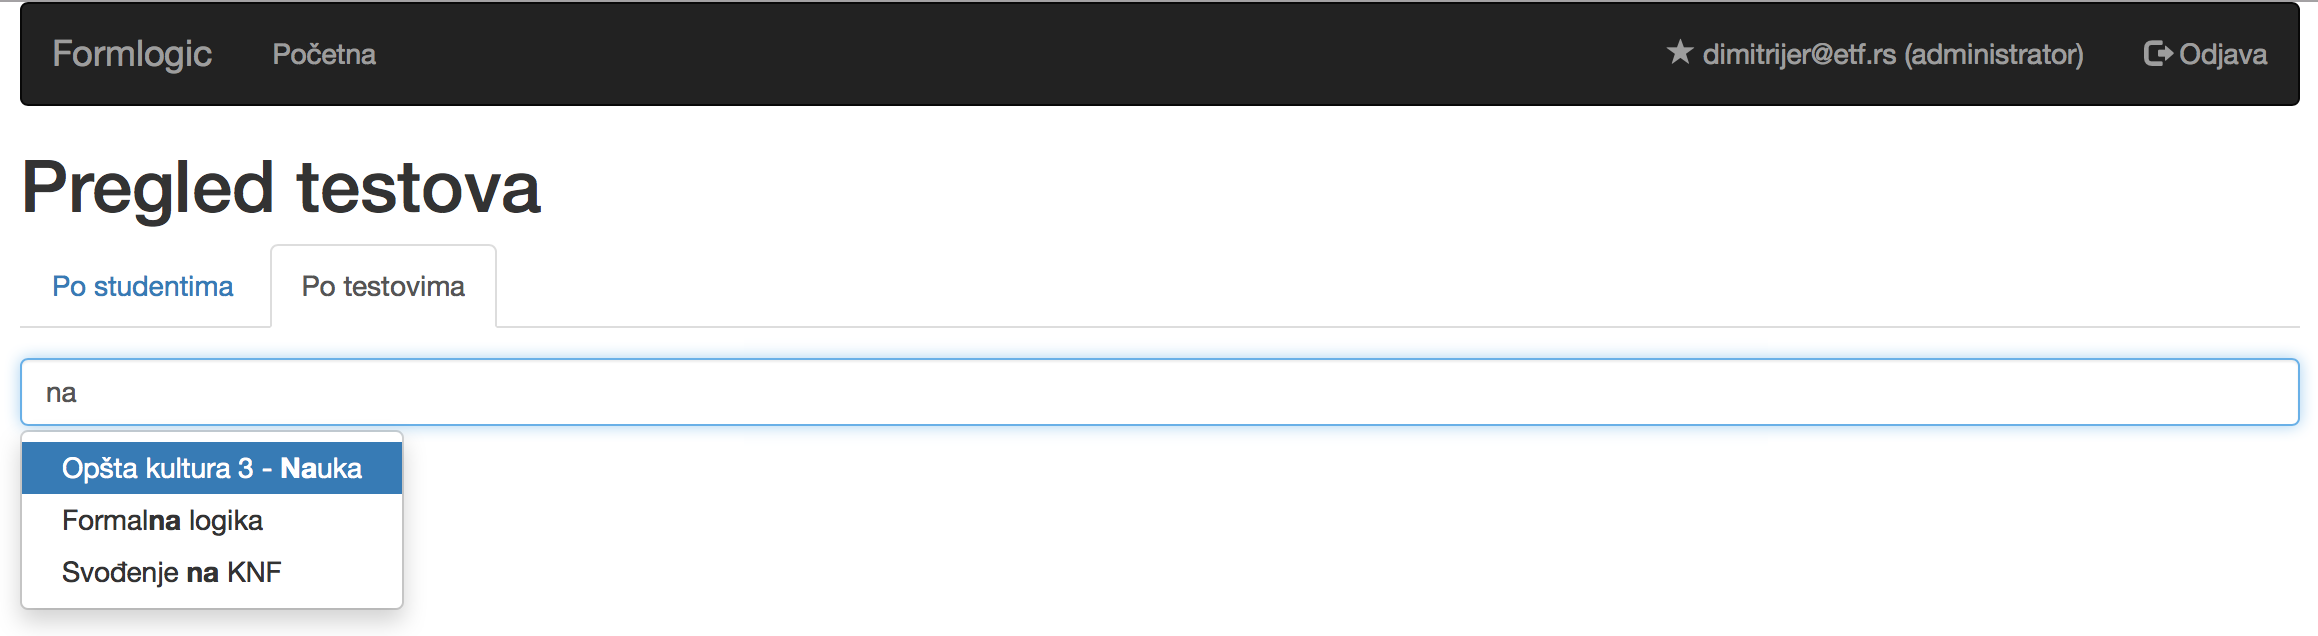
\includegraphics[width=0.95\textwidth]{assignments-admin-tests}}
\caption{Dinamičko sužavanje izbora pretrage tokom kucanja, \textit{gore}: primer pretrage preko email naloga studenata, \textit{dole}: primer pretrage preko imena testa}
\label{fig:assignments-admin}
\end{figure}

Tokom unošenja email naloga, ili imena testa, prilikom pretrage, izbor se dinamički sužava, tako da je dovoljno otkucati samo mali broj karaktera kako bi se prikazao željeni izbor. Stavke koje odgovaraju upitu se prikazuju u padajućoj listi, a kroz prikazane stavke se može kretati strelicama gore i dole. Izabrana stavka iz liste se potvrđuje pritiskom na taster Enter, a može se odabrati i klikom. Nakon potvrđivanja izbora, server vraća sve odrađene testove (instance testova koje su predate, pogledati sekciju \ref{section:submit}, i ti rezultati se prikazuju u tabelarnom obliku, ispod formulara za pretragu. Za svaki odrađen test prikazuje se ime testa, email nalog studenta, vreme početka i kraja izrade, ocena u obliku procenta pitanja na koja je student dao tačan odgovor, i, najzad, link za pregled testa (slika \ref{fig:assignments-admin-results}).
\begin{figure}[h]
\centering
\fbox{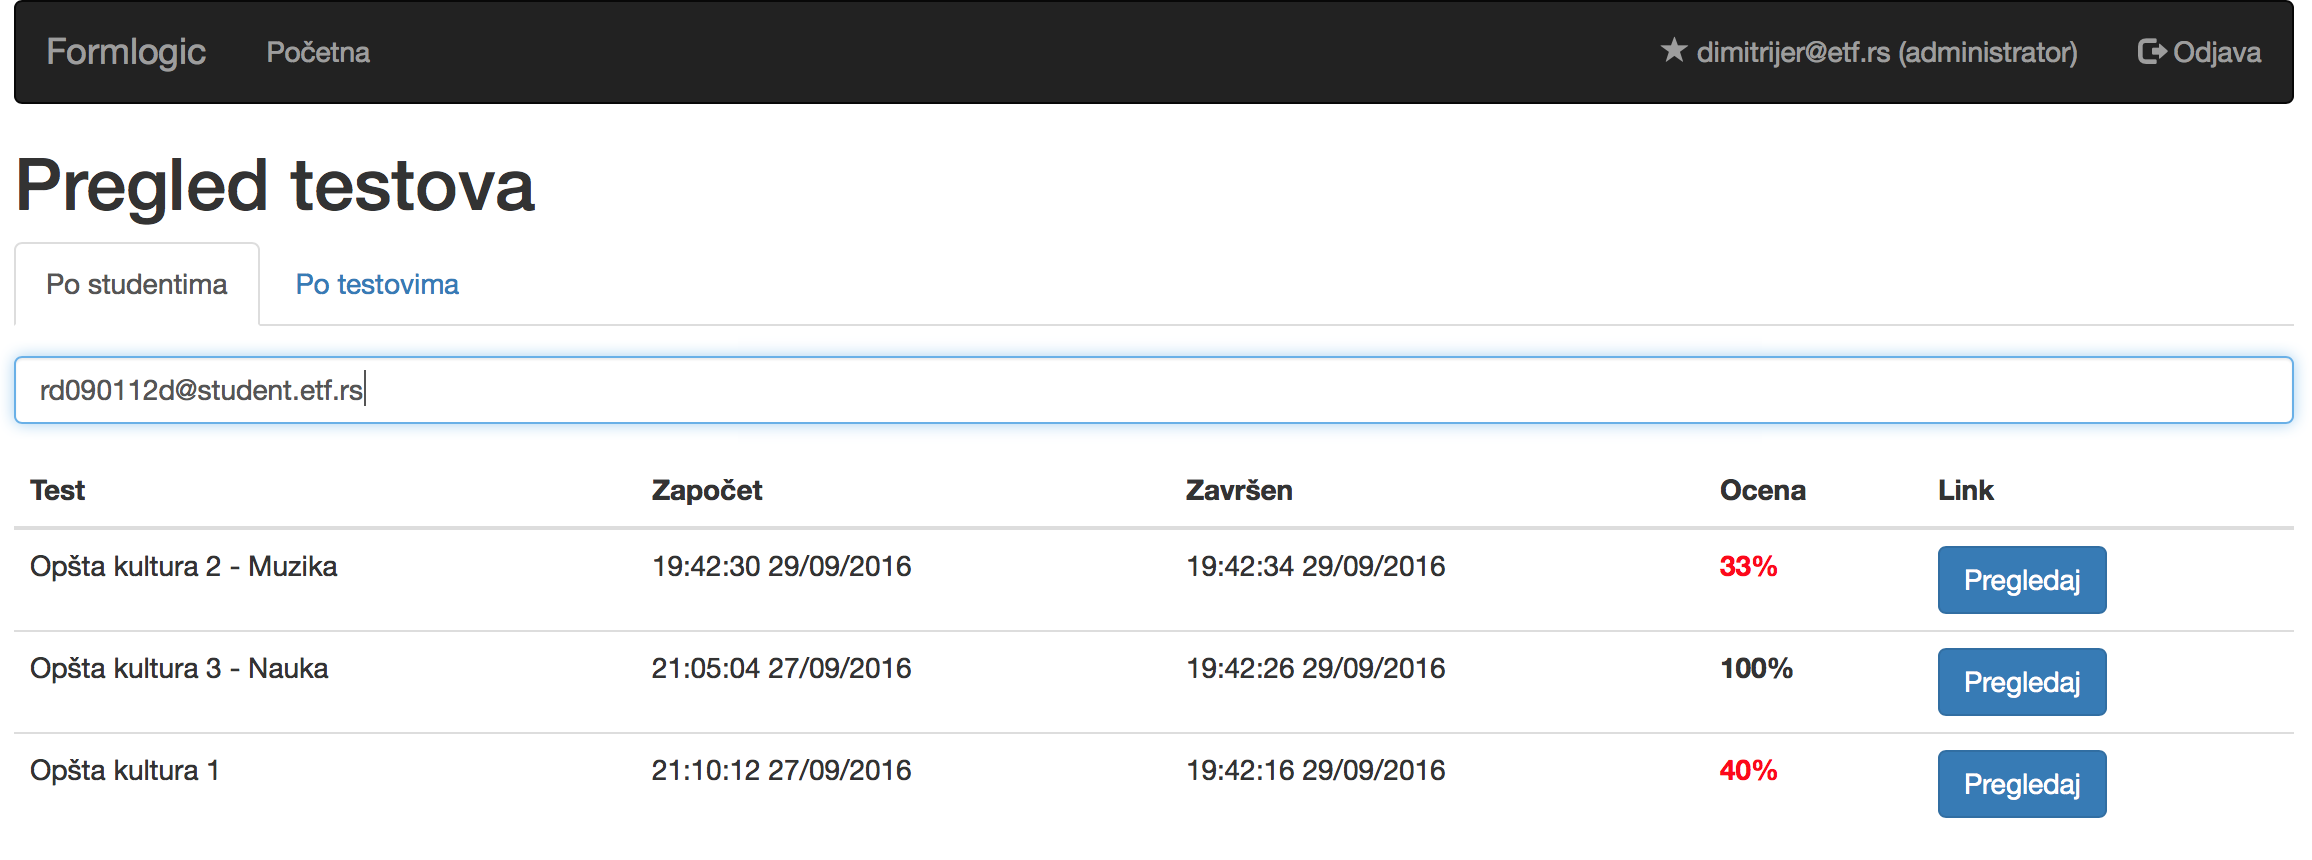
\includegraphics[width=0.95\textwidth]{assignments-admin-student-results}}
\fbox{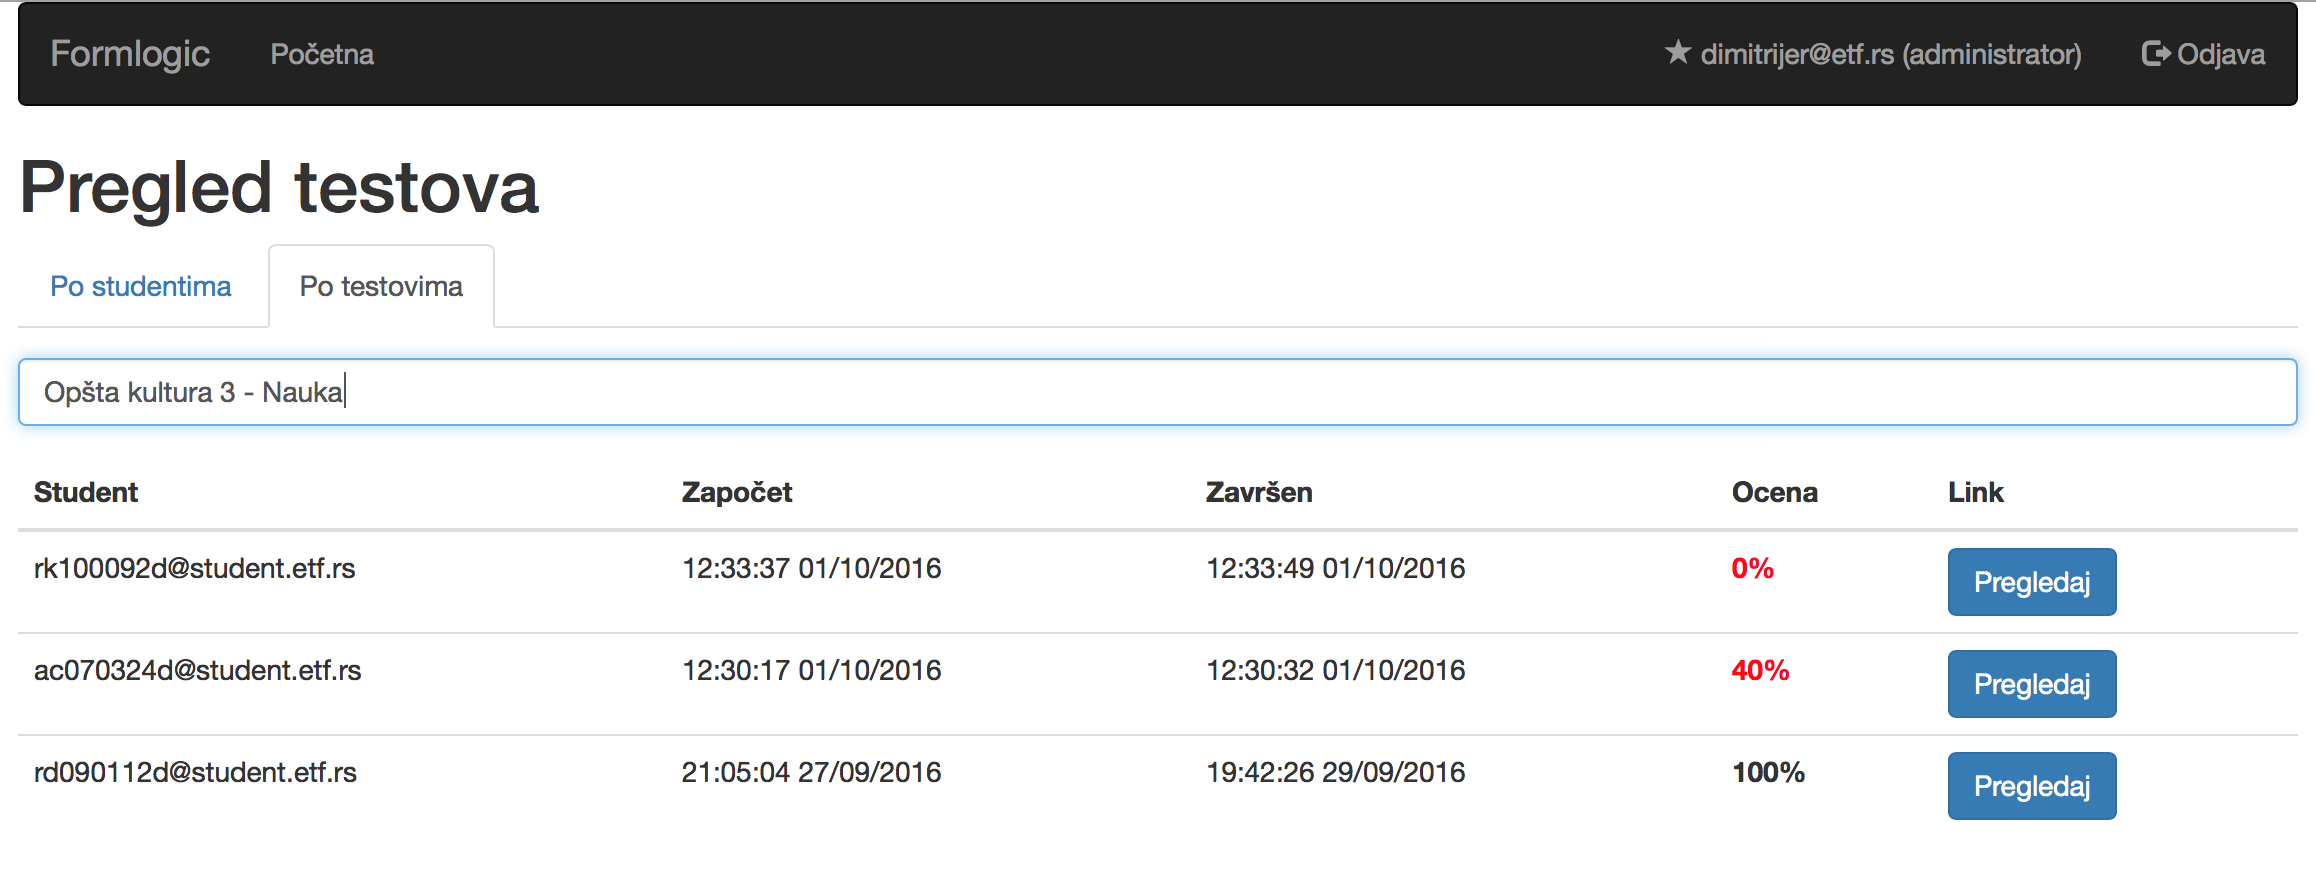
\includegraphics[width=0.95\textwidth]{assignments-admin-test-results}}
\caption{\textit{Gore}: primer rezultata pretrage preko email naloga studenata, \textit{dole}: primer rezultata pretrage preko imena testa}
\label{fig:assignments-admin-results}
\end{figure}

\subsection{Pregled i izmena ocene završenog testa}
Nakon što administrator odabere jedan od testova za pregled, prikazuje se stranica koja je identična stranici iz sekcije \ref{section:submit} (čak je i URI isti), sa nekoliko razlika (slika \ref{fig:task-admin}, uporediti sa slikom \ref{fig:task}).
\begin{figure}[h]
\centering
\fbox{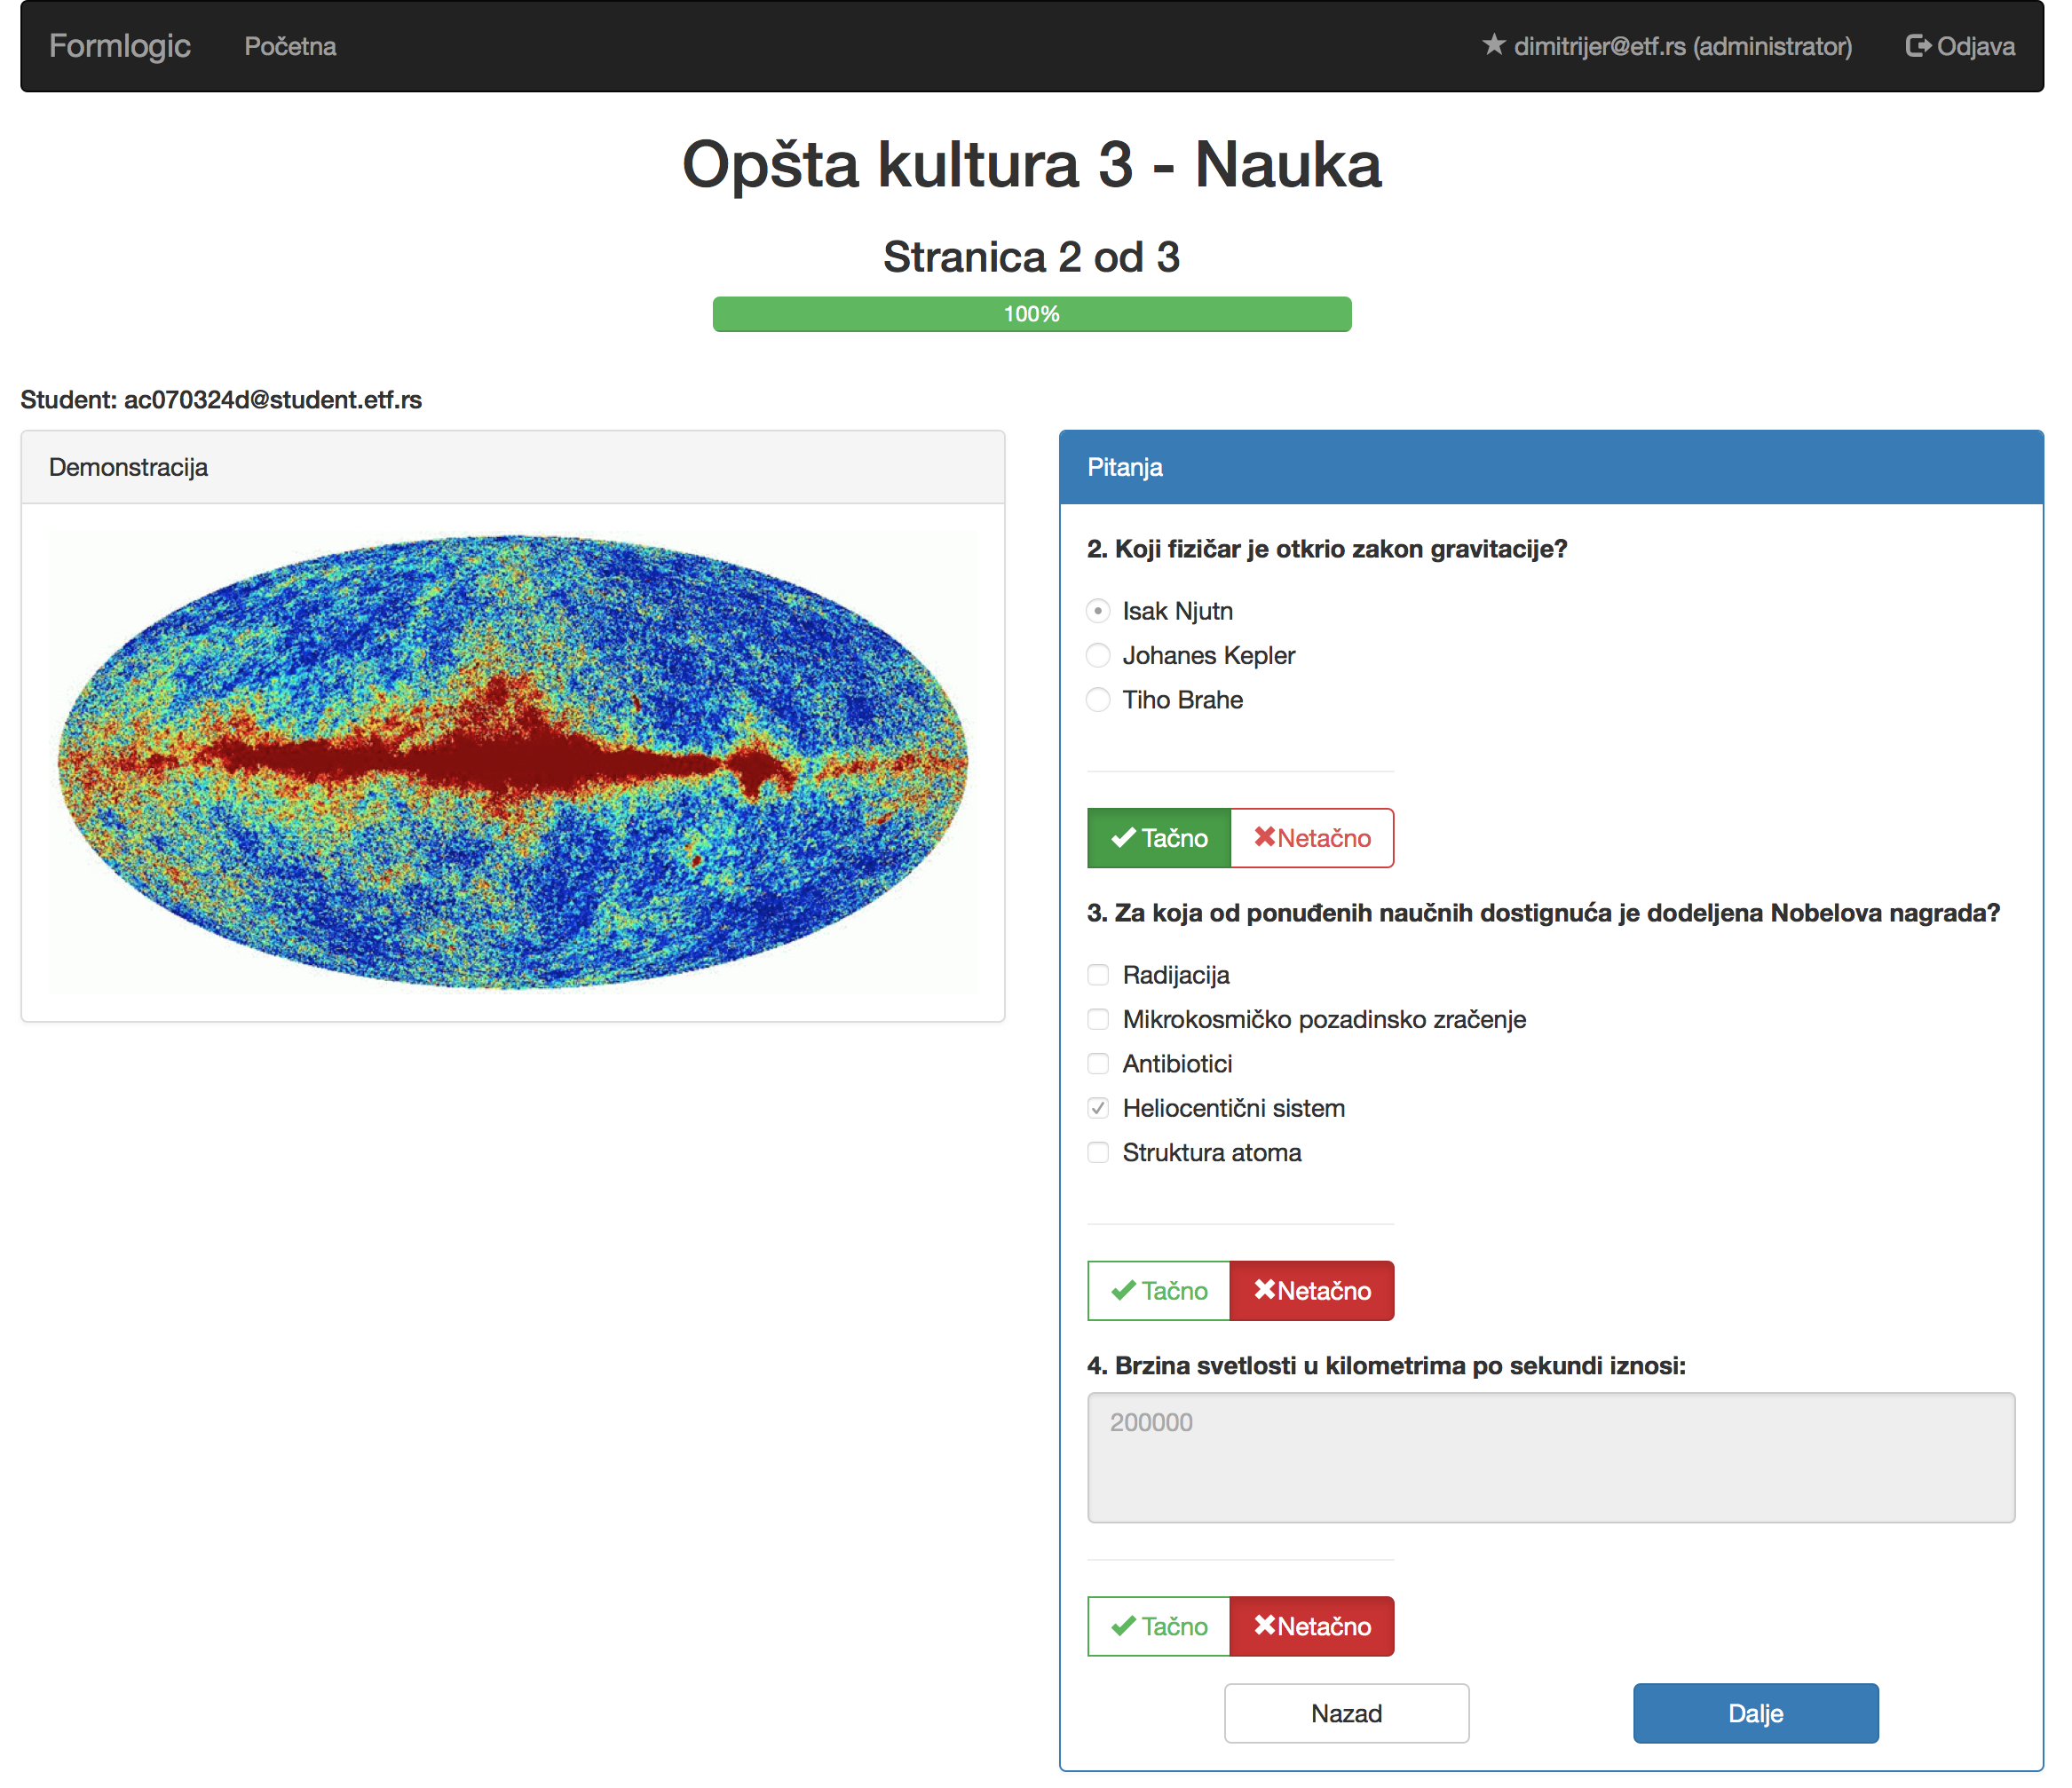
\includegraphics[width=0.95\textwidth]{task-admin}}
\caption{Izgled stranice za pregled testa - izmena ocene za odgovor se vrši izborom jednog od dva radio dugmeta ispod svakog odgovora}
\label{fig:task-admin}
\end{figure}
Prva razlika je u tome što administratoru nije dozovljeno da menja odgovore koje je student dao - sve kontrole formulara su onemogućene. Ovim se garantuje da originalni odgovori ne mogu biti menjani nakon što student preda test. Takođe, pri vrhu stranice se prikazuje email nalog studenta koji je predao test.

Još jedna razlika je u tome što se na ovoj stranici nakon svakog pitanja prikazuje automatski dodeljena\emph{ocena} za to pitanje. Ocena je jedna obična Bulova vrednost koju sistem dodeljuje svakom odgovoru nakon što student preda test, i označava da li se odgovor na pitanje prihvata kao tačan, ili odbacuje kao netačan odgovor. Administrator može da menja ovu vrednost za svako pitanje po svom nahođenju, i time utiče na konačnu ocenu testa, u vidu procenta uspešnosti. Kako je za pitanja sa jednim ili više ponuđenih odgovora automatsko ocenjivanje trivijalno, ova funkcionalnost se uglavnom koristi za pitanja na koje odgovor treba dati u slobodnoj formi, gde je mogućnost sistema da korektno oceni odgovor ograničena. Tada administrator može odlučiti da je student dao tačan odgovor tamo gde je sistem procenio da odgovor nije bio tačan, ili obratno.

Administrator se kreće kroz stranice sa pitanjima na isti način kao student, s tim što se na poslednjoj stranici mesto dugmeta \textbf{Predaj} nalazi dugme \textbf{Kraj}. Klik na ovo dugme administratora vodi na početnu stranicu. Bitno je napomenuti da se ovim ne menja zapisan datum predaje testa. Ovo predstavlja finalnu razliku u odnosu na funkcionalnost stranice kada joj pristupa student.

\subsection{Dodavanje novih testova}
\label{sec:panel-contents}
Kako se dodavanje novih testova radi ubacivanjem novih redova u bazi, prvo je neophodno prikazati i objasniti entitete u bazi vezane za testove i relacije između njih (slika \ref{fig:db}).
\begin{figure}[p]
\centering
\begin{tikzpicture}
\node[entity] (a) at (0,0) {
static.\textbf{assignment}
\nodepart{second}
\begin{tabularx}{4cm}{X X}
\underline{\textbf{id}} \hfill & \hfill \texttt{int4} \\
name \hfill & \hfill \texttt{text} \\
category \hfill & \hfill \texttt{text} \\
\end{tabularx}
};

\node[entity, right=of a] (t) {
static.\textbf{task}
\nodepart{second}
\begin{tabularx}{5.5cm}{X X}
\underline{\textbf{id}} \hfill & \hfill \texttt{serial} \\
assignment\_id \hfill & \hfill \texttt{int4} \\
ord \hfill & \hfill \texttt{int4} \\
contents \hfill & \hfill \texttt{text} \\
\end{tabularx}
};

\node[entity, below=of t] (q) {
static.\textbf{question}
\nodepart{second}
\begin{tabularx}{7cm}{X X}
\underline{\textbf{id}} \hfill & \hfill \texttt{serial} \\
task\_id\hfill & \hfill \texttt{int4} \\
ord \hfill & \hfill \texttt{int4} \\
type \hfill & \hfill \texttt{question\_type} \\
body \hfill & \hfill \texttt{text} \\
choices \hfill & \hfill \texttt{text[]} \\
answers \hfill & \hfill \texttt{int2[]} \\
\end{tabularx}
};

\draw[dashed,-{Latex[length=3mm]}, thick] (a) -- (t);
\draw[dashed,-{Latex[length=3mm]}, thick] (t) -- (q);
\end{tikzpicture}
\caption{Entiteti koji opisuju testove i relacije među njima}
\label{fig:db}
\end{figure}
\begin{description}
\item [\textbf{Assignment}] je entitet na vrhu hijerarhije koji predstavlja jedan test. On sadrži ime i kategoriju testa. Primarni ključ se navodi prilikom ubacivanja u bazu.
\item [\textbf{Task}] je entitet koji predstavlja stranicu jednog testa. Ovaj entitet ima egzistencijalnu zavisnost od \textbf{Assignment} entiteta, koja se modeluje stranim ključem u vidu kolone \texttt{assignment\_id}. Sadrži redni broj unutar testa i opcioni sadržaj panele sa demonstracijom. Primarni ključ se generiše automatski, inkrementiranjem sekvence.
\item [\textbf{Question}] predstavlja jedno pitanje u okviru stranice testa. Ima egzistencijalnu zavisnost od \textbf{Task} entiteta (kolona \texttt{task\_id}). Sadrži redni broj unutar stranice testa, tip pitanja, telo pitanja, ponuđene odgovore u vidu niza stringova, i niz celih brojeva koji označavaju indekse \emph{tačnih} odgovora unutar niza ponuđenih odgovora. Primarni ključ se takođe generiše automatski, inkrementiranjem sekvence. Prilikom ubacivanja reda se proverava da li su indeksi u koloni \texttt{answers} u validnom opsegu koji je definisan brojem elemenata u \texttt{choices} tabeli.
\end{description}

Prema ovome, dodavanje novih testova svodi se na ubacivanje novog reda koji predstavlja test u \texttt{assignment} tabelu, ubacivanje novog reda za svaku stranicu u testu u \texttt{task} tabelu, i ubacivanje svih pitanja po stranici u \texttt{question} tabelu. Takođe je bitno napomenuti da se sve ove tabele nalaze u \texttt{static} shemi, gde su odvojene sve tabele koje se ne menjaju tokom izvršavanja aplikacije. Primer ubacivanja testa sa slike \ref{fig:task} je priložen u listingu \ref{lst:insert}.
\lstinputlisting[float, floatplacement=p, caption=Primer dodavanja jednog testa sa jednom stranicom i tri pitanja, label=lst:insert, language=SQL]{listings/assignment-example.sql}

Kako bi automatsko ocenjivanje radilo i za odgovore u slobodnoj formi, za takva pitanja autor preporučuje da se u \texttt{choices} kolonu ubace tačni odgovori u što više mogućih formi, a da se u \texttt{answers} koloni navedu svi indeksi iz \texttt{choices} niza.